\documentclass[12pt]{article}
\usepackage{charter} % font
\usepackage[margin=1in]{geometry} % margin
\usepackage{hyperref} % hyperlinks
\usepackage{enumitem} % Enumeration
\usepackage{graphicx} % images
\usepackage{float} % image placement
\graphicspath{ {.} } 

%%%%%%%%%%%%%%%%%%%%%%%%%%%%%%%%%%%%%%%%%%%%%%%%%%%%%%%%%%%%%%%%%%%%%%%%%%%%%%%%

\title{%
	\textbf{Assignment 3 \\ 
	Sorting: Putting your affairs in order \\
	\large WRITEUP} }

	\author{Zack Traczyk \\ CSE13S - Spring 2021}
	\date{Due: April 25\textsuperscript{th} at 11:59 pm}

%%%%%%%%%%%%%%%%%%%%%%%%%%%%%%%%%%%%%%%%%%%%%%%%%%%%%%%%%%%%%%%%%%%%%%%%%%%%%%%%

	\begin{document}

	\maketitle

	\section{Time Complexity}

	In this assignment, four sorting algorithms were implemented:
	Bubble Sort, Shell Sort, Quicksort with a stack, and Quicksort with a queue.
	Each algorithm has a different balance of memory usage, comparisons, and swamps resulting in different runtime and Big-$O$ analyses.
	Since the length of the array will be discussed often, this value will be referred to as $n$.

%%%%%%%%%%%%%%%%%%%%%%%%%%%%%%%%%%%%%%%%%%%%%%%%%%%%%%%%%%%%%%%%%%%%%%%%%%%%%%%%

	\subsection{Bubble Sort}

	Bubble Sort is relatively naive sort, simply switching bordering values until the array is sorted.
	Unsurprisingly, this approach is not efficient for larger arrays.
	Bubble Sort had the worst time complexity out of all the sorts implemented.
	Figure \ref{bubble} displays the relationship between the amount of comparisons the algorithm performs for $n$ values.
	Bubble Sort's comparisons increase exponentially as $n$ resulting in a time complexity of $O(n^2)$.

	A reversed array requires the most amount of comparisons in bubble sort. Since the items bubble to the top,

	The corresponding $C$ value for bubble sort is 

	\begin{figure}[H]
		\caption{Bubble Sort}\label{bubble}
		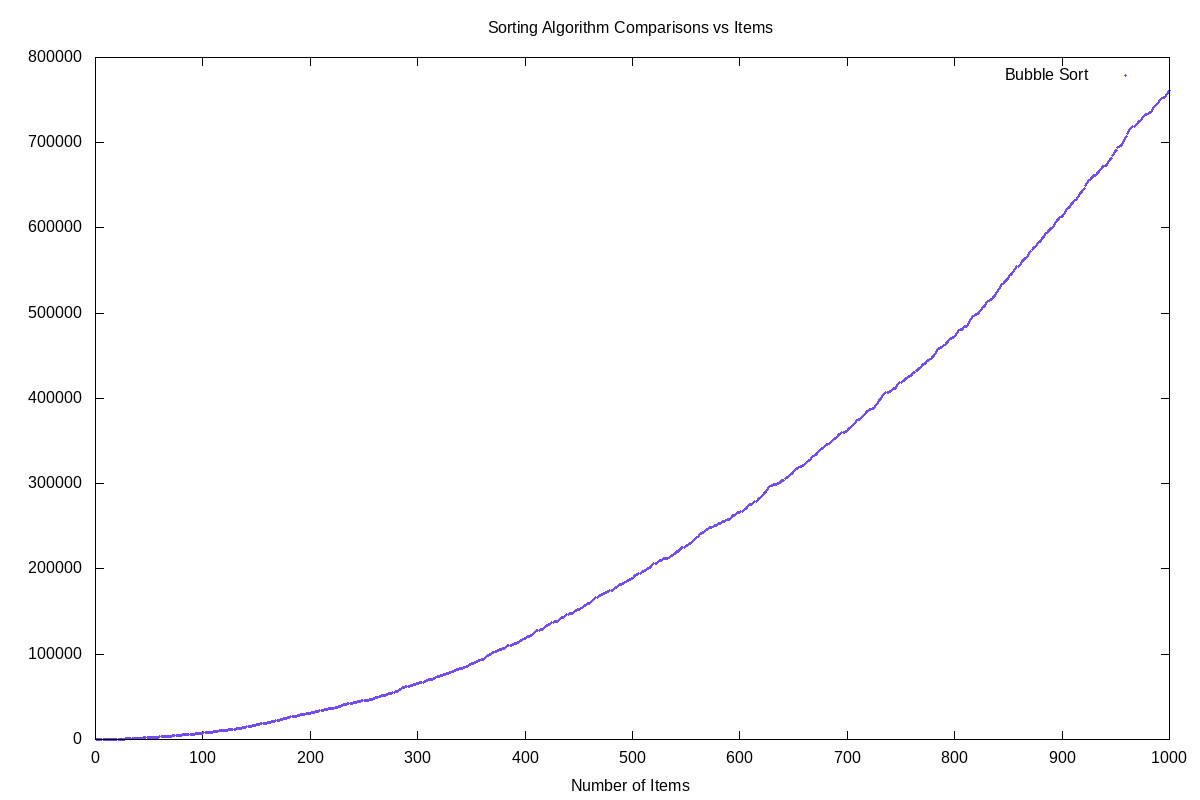
\includegraphics[width=6in]{bubble}
		\centering
	\end{figure}

%%%%%%%%%%%%%%%%%%%%%%%%%%%%%%%%%%%%%%%%%%%%%%%%%%%%%%%%%%%%%%%%%%%%%%%%%%%%%%%%

	\subsection{Shell Sort}

	Shell sort preformed much better than Bubble Sort.
	Just by looking at figure \ref{shell} the curve is obviously less slopped than figure \ref{bubble}.
	A generic shell sort algorithm's worst case scenario is $O(n^2)$.
	However this is because the gap size is 1, equivalent to bubble sort.
	This implementation uses a Pratt sequence of gaps.
	This results in a time complexity of $O(n log n)$.

	Reverse

	\begin{figure}[H]
		\caption{Shell Sort}\label{shell}
		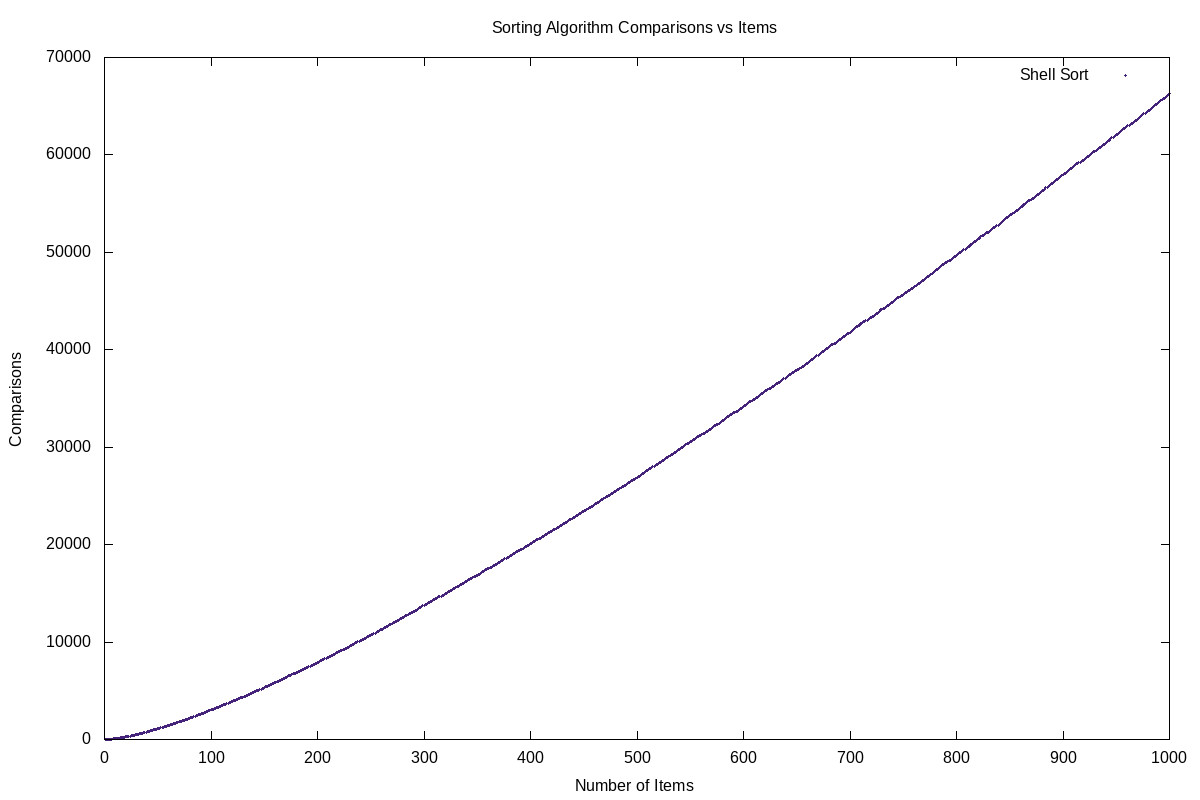
\includegraphics[width=6in]{shell}
		\centering
	\end{figure}

%%%%%%%%%%%%%%%%%%%%%%%%%%%%%%%%%%%%%%%%%%%%%%%%%%%%%%%%%%%%%%%%%%%%%%%%%%%%%%%%

	\subsection{Quicksort}

	Quick sort preformed the best by far. Figure \ref{stack}. Figure \ref{queue}.

	\begin{figure}[H]
		\caption{Quicksort (Stack)}\label{stack}
		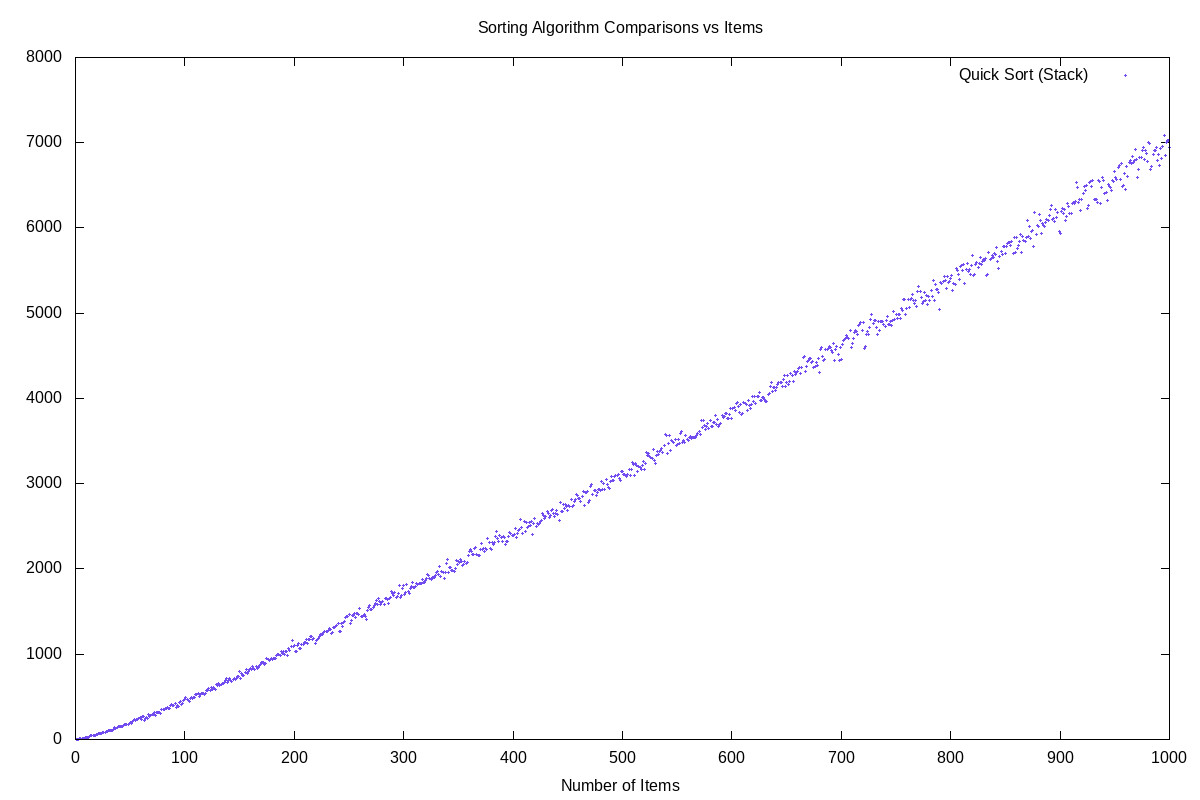
\includegraphics[width=\textwidth]{quick_stack}
		\centering
	\end{figure}

	\begin{figure}[H]
		\caption{Quicksort (Queue)}\label{queue}
		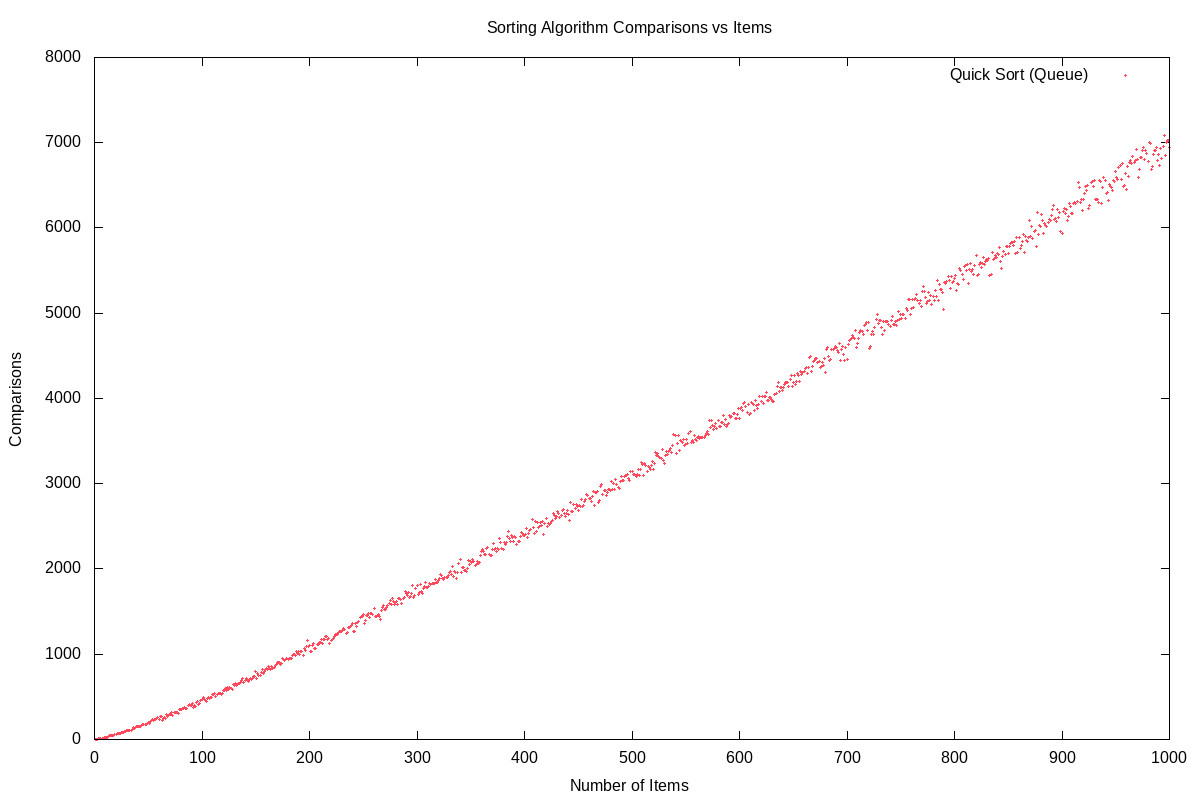
\includegraphics[width=\textwidth]{quick_queue}
		\centering
	\end{figure}[h]

	There is a linear relationship between the size of the array that is being sorted and the size of the resulting queue/ stack. This is because the queue/ stack is initialized as the $2n$.

	When looking at size figure \ref{quick_size}.

	\begin{figure}[H]
		\caption{Quicksort Data Structure Size Comparison}\label{quick_size}
		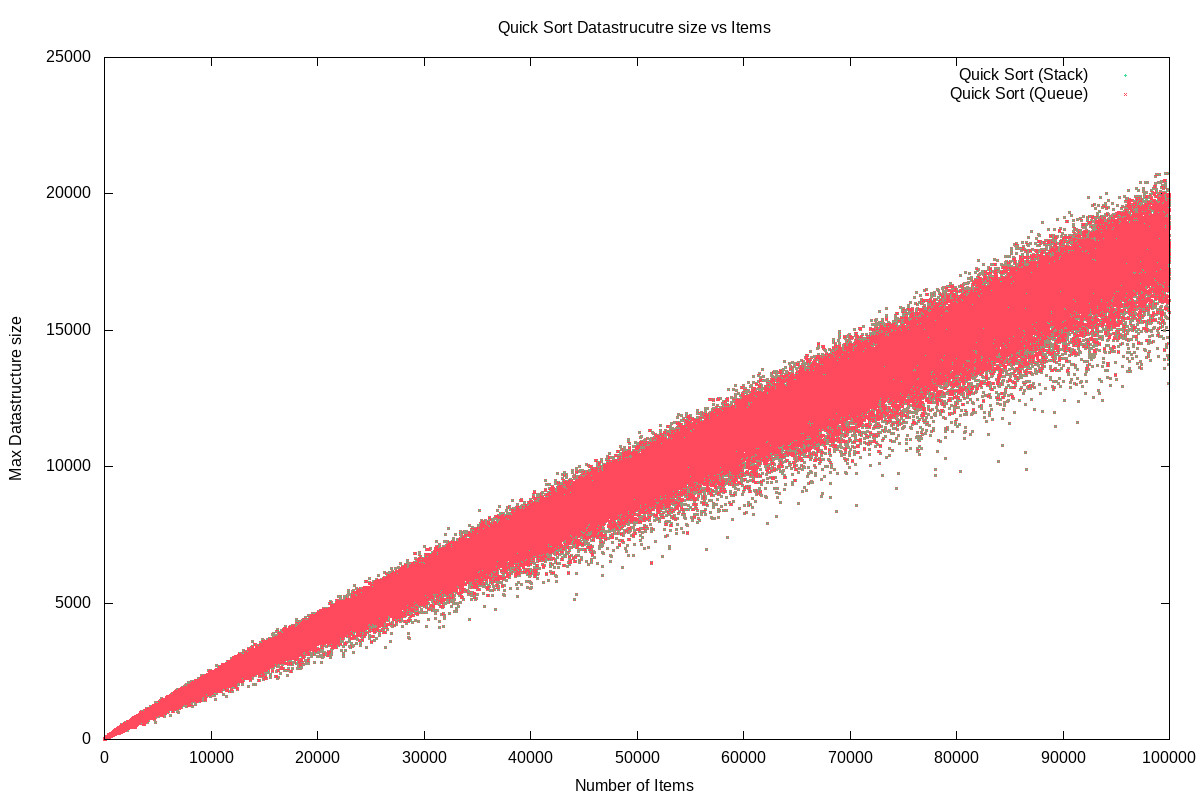
\includegraphics[width=\textwidth]{quick_comparison_size}
		\centering
	\end{figure}

%%%%%%%%%%%%%%%%%%%%%%%%%%%%%%%%%%%%%%%%%%%%%%%%%%%%%%%%%%%%%%%%%%%%%%%%%%%%%%%%

	\subsection{Overall}

	As I stated, overall figure \ref{comparison}.

	\begin{figure}[H]
		\caption{Overall Comparison}\label{comparison}
		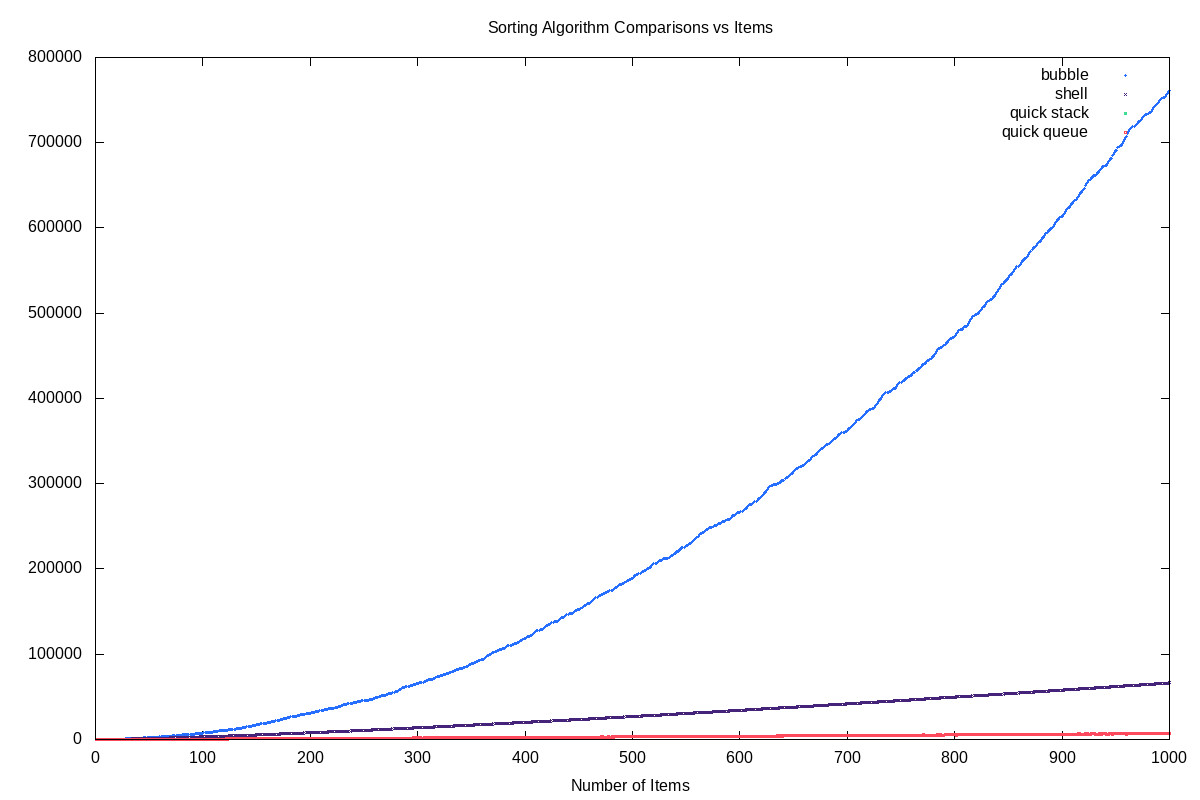
\includegraphics[width=\textwidth]{comparison}
		\centering
	\end{figure}

%%%%%%%%%%%%%%%%%%%%%%%%%%%%%%%%%%%%%%%%%%%%%%%%%%%%%%%%%%%%%%%%%%%%%%%%%%%%%%%%

	\section{What I Learned}

	Picking the right algorithm is crucial for accomplishing fast code. Furthermore, right does not necessarily mean smallest Big-$O$ or even the fastest. It is about considering memory usage, and size of array.

	\end{document}

